\documentclass[letterpaper,12pt]{article}
\usepackage[margin=64pt]{geometry}
\usepackage{amsthm}
\usepackage{amsmath}
\usepackage{amssymb}
\usepackage{parskip}
\usepackage{graphicx}
\usepackage{enumerate}
\usepackage{hyperref}
\usepackage{listings}
\newcommand{\transpose}{^{\mbox{\tiny T}}}


\begin{document}
\thispagestyle{empty}

\hrule \vspace{0.5em}
\noindent {\bf CFRM 462: Introduction to Computational Finance and Econometrics} \hfill Homework 3 \newline \hrule

\vspace{1em}

\begin{enumerate}
\item 
\subitem{a)} 
\begin{lstlisting}
        A = matrix(
        c(1,4,7,
        2,4,8,
        6,1,3), nrow = 3, ncol = 3, byrow = TRUE)
        
        B = matrix(c(4,4,0,5,9,1,2,2,5), nrow = 3, 
                ncol = 3, byrow = TRUE)
        
        x = matrix(c(1,2,3), nrow = 3, ncol = 1)
        y = matrix(c(5,2,7), nrow = 3, ncol = 1)
\end{lstlisting}

\subitem{b)}
\begin{lstlisting}
        > t(A)
             [,1] [,2] [,3]
        [1,]    1    2    6
        [2,]    4    4    1
        [3,]    7    8    3
        > t(B)
             [,1] [,2] [,3]
        [1,]    4    5    2
        [2,]    4    9    2
        [3,]    0    1    5
        > t(x)
             [,1] [,2] [,3]
        [1,]    1    2    3
        > t(y)
             [,1] [,2] [,3]
        [1,]    5    2    7
\end{lstlisting}

\subitem{c)}
\begin{lstlisting}
        > A+B
             [,1] [,2] [,3]
        [1,]    5    8    7
        [2,]    7   13    9
        [3,]    8    3    8
        > A-B
             [,1] [,2] [,3]
        [1,]   -3    0    7
        [2,]   -3   -5    7
        [3,]    4   -1   -2
        > 2*A
             [,1] [,2] [,3]
        [1,]    2    8   14
        [2,]    4    8   16
        [3,]   12    2    6
        > A%*%x
             [,1]
        [1,]   30
        [2,]   34
        [3,]   17
        > t(y)%*%A%*%x
             [,1]
        [1,]  337
\end{lstlisting}

\subitem{d)}

\begin{lstlisting}
        x = seq(-1,2,length = 100)
        plot(x,1-x, lwd=2, ylab="y", type = "l",col = "red",
            main = "Linear System")
        
        abline(a=0.5, b=-0.5, lwd=2)
        abline(h = 0,v=0)
\end{lstlisting}
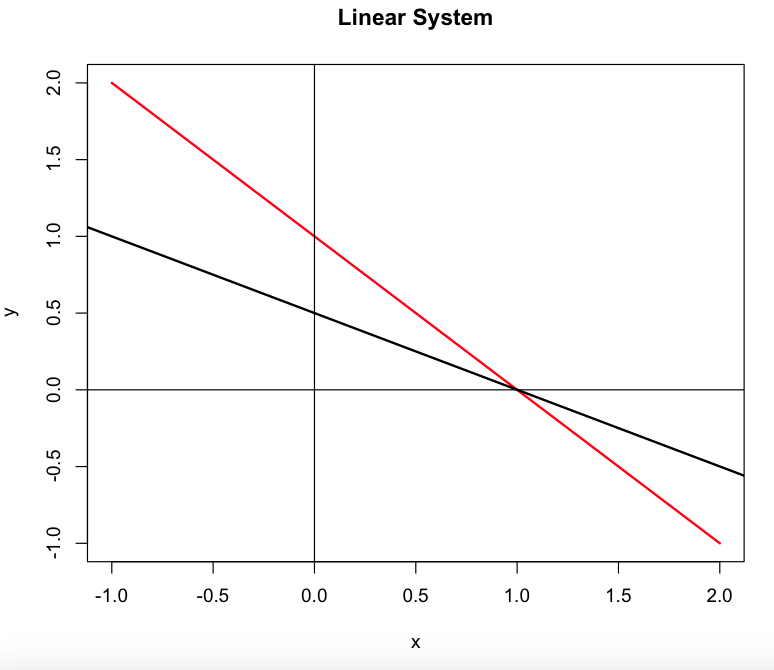
\includegraphics[scale = 0.5]{lines}

\subitem{e)}
\begin{lstlisting}
        > matA = matrix(c(1,1,2,4), 2, 2, byrow=TRUE)
        > vecB = c(1,2)
        > matA.inv = solve(matA)
        > matA.inv
             [,1] [,2]
        [1,]    2 -0.5
        [2,]   -1  0.5
        > matA.inv%*%matA
             [,1] [,2]
        [1,]    1    0
        [2,]    0    1
        > matA%*%matA.inv
             [,1] [,2]
        [1,]    1    0
        [2,]    0    1
        > z = matA.inv%*%vecB
        > z
             [,1]
        [1,]    1
        [2,]    0
        > 
        > mu = matrix(c(0.01,0.04,0.02),nrow = 3, ncol = 1)
        > 
        > sigma = matrix(c(0.1,0.3,0.1,0.3,0.15,-0.2
        + ,0.1,-0.2,0.08), nrow = 3, ncol = 3, byrow = TRUE)
        > 
        > #expected value
        > w = c(rep(1/3,3))
        > e.x = crossprod(w,mu)
        > 
        > t(w) %*% sigma %*% w
               [,1]
        [1,] 0.0811
\end{lstlisting}
\item Simulating Time Series Data
\subitem{a)}
\begin{lstlisting}
        #Simulate a MA(1) model Y_t = 0.05 + e_t + theta * e_t-1 
        #where e(t) ~ N(0,0.1^2)
        set.seed(123)
        mu = 0.05
        e = rnorm(n.obs, mean = 0, sd = 0.1)
        theta = list(ma = 0.5)
        y.1 = mu + arima.sim(model = theta, n = 250, mean = 0, sd = 0.1)
        
        set.seed(123)
        theta = list(ma = 0.9)
        y.2 = mu + arima.sim(model = theta, n = 250, mean = 0, sd = 0.1)
        
        #Plot Y_t
        par(mfrow = c(2,1))
        ts.plot(y.1, main = "MA(1) Process: mu = 0.05, theta = 0.5", 
        		xlab = "time", ylab = "y(t)")
        
        plot(y.2, main = "MA(1) Process: mu = 0.05, theta = 0.9", 
        		xlab = "time", ylab = "y(t)")
\end{lstlisting}
\includegraphics[scale = 0.5]{ma1}

The data looks stationary and tends towards the mean.

\subitem{b)}
\begin{lstlisting}
        > mean(y.1)
        [1] 0.0488
        > mean(y.2)
        [1] 0.0484
\end{lstlisting}

\subitem{c)}
\begin{lstlisting}
	> var(y.1)
	[1] 0.0106
	> var(y.2)
	[1] 0.0151
\end{lstlisting}

\subitem{d)}
	\begin{lstlisting}
	ma.acf1 = ARMAacf(ar = 0, ma = 0.5, lag.max = 10)
	ma.acf2 = ARMAacf(ar = 0, ma = 0.9, lag.max = 10)

	#Plot ACFs
	par(mfrow = c(2,1))
	plot(0:10,ma.acf1, type = "h", lwd = 2, col = "blue", 
		xlab = "lag", ylab = "rho(j)", 
		main = "ACF for MA(1): theta = 0.5")

	plot(0:10,ma.acf2, type = "h", lwd = 2, col = "blue", 
		xlab = "lag", ylab = "rho(j)", 
		main = "ACF for MA(1): theta = 0.9")	
	\end{lstlisting}    

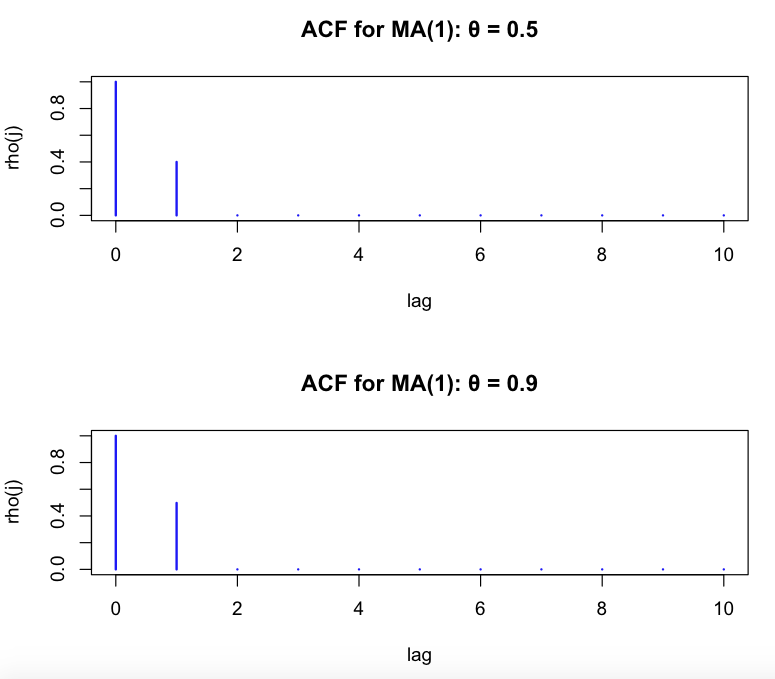
\includegraphics[scale = 0.5]{MACF1}

\subitem{a)}
	\begin{lstlisting}
	set.seed(123)

        ar1 = mu + arima.sim(model = list(ar = 0.5),
                n = 250, mean = 0, sd = 0.1)
        
        ar2 = mu + arima.sim(model = list(ar = 0.9), 
                n = 250, mean = 0, sd = 0.1)
        
        #Plot AR
        par(mfrow = c(2,1))
        ts.plot(ar1, main = "MA(1) Process: mu = 0.05, 
                phi = 0.5", xlab = "time", ylab = "y(t)")
        ts.plot(ar2, main = "MA(1) Process: mu = 0.05, 
                phi = 0.9", xlab = "time", ylab = "y(t)")        		
	\end{lstlisting} 

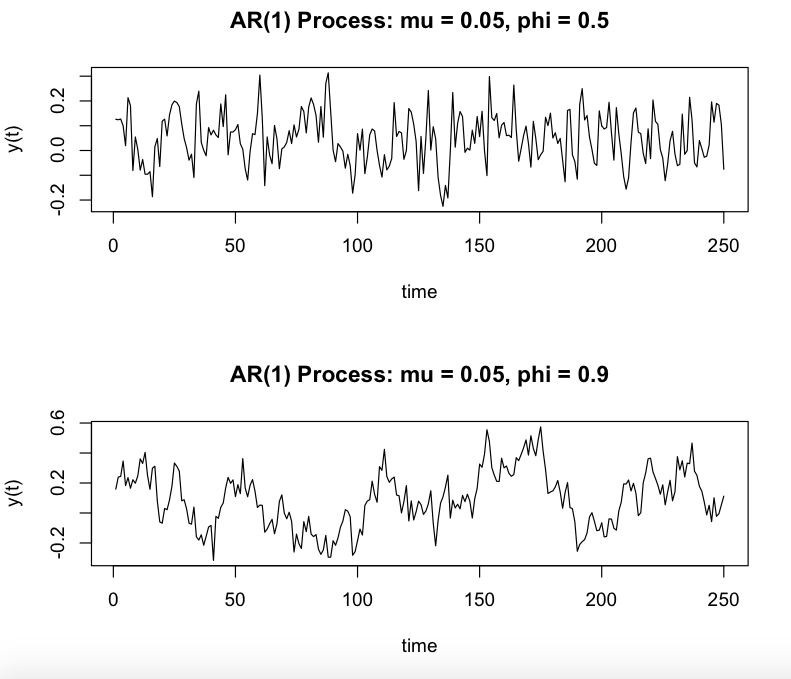
\includegraphics[scale =0.5]{AR1}

\subitem{b)}
	\begin{lstlisting}
	> mean(ar1)
        [1] 0.0481
        > mean(ar2)
        [1] 0.0937
	\end{lstlisting}           

\subitem{c)}
	\begin{lstlisting}
        > var(ar1)
        [1] 0.0105
        > var(ar2)
        [1] 0.0354
	\end{lstlisting}
	
\subitem{d)}
	\begin{lstlisting}
	ar.acf1 = ARMAacf(ar = 0.5, ma = 0, lag.max = 10)
        ar.acf2 = ARMAacf(ar = 0.9, ma = 0, lag.max = 10)
        
        par(mfrow = c(2,1))
        plot(0:10,ar.acf1, type = "h", lwd = 2, col = "blue", 
                xlab = "lag", ylab = "rho(j)", 
                main = "ACF for AR(1): ? = 0.5")
        
        plot(0:10,ar.acf2, type = "h", lwd = 2, col = "blue", 
                xlab = "lag", ylab = "rho(j)", 
                main = "ACF for AR(1): ? = 0.9")
	\end{lstlisting}
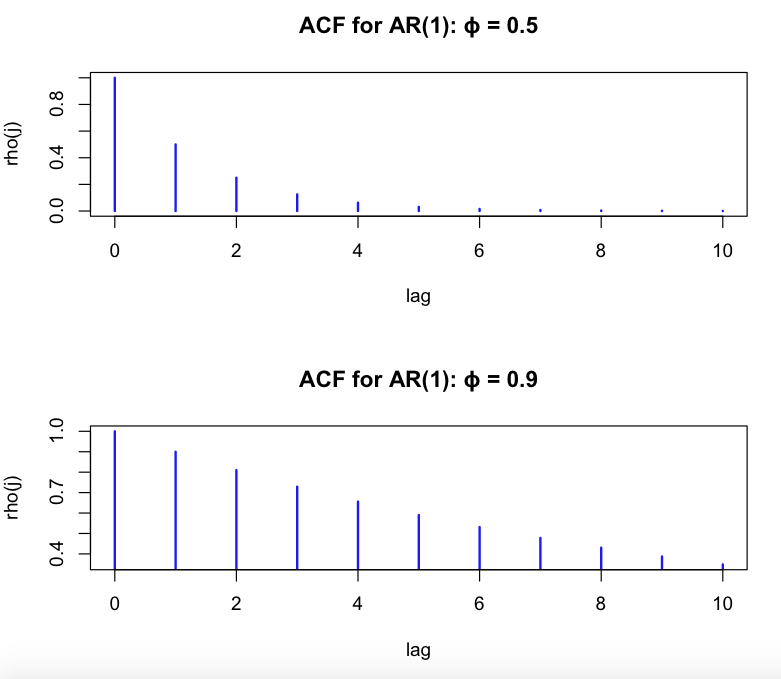
\includegraphics[scale = 0.5]{ARCF1}
\item Ruppert and Matteson Excercises
\subitem{9)} 
	\begin{lstlisting}
	data = read.csv('~/Documents/CFRM 462/
            	datasets/MCD_PriceDaily.csv')
        head(data)
        adjPrice = data[ , 7]
        plot(adjPrice, type = "l", lwd = 2)
	\end{lstlisting}
	It is not stationary because there is no reversion to the mean
	
\subitem{10)}
	\begin{lstlisting}
	n = length(adjPrice)
        logRet = log(adjPrice[-1]/adjPrice[-n])
        date = as.Date(data[,1],"%m/%d/%Y")
        plot(date[-1],logRet, xlab = "Date", ylab = "Return",
                main = "McDonalds Log Returns", type = "l")
        
        hist(logRet, 80, freq= FALSE)
        qqnorm(logRet)
        qqline(logRet)
	\end{lstlisting}

\subitem{11)}
No the log returns do not appear to be normally distributed.  The log returns may appear Gaussian at first, but closer examination of the tails may prove otherwise. There are heavy bins on the left section of the tail and the tails are very long. They do appear nearly symmetric, but the left tail seems heavy and longer compared to the right tail.

\item Chapter 12.16 Problems 3 \& 4
\subitem{3)} $Y_t = 5 - 0.55 Y_{t-1} + \epsilon_t$
No this is not a stationary process because the roots of the polynomial must be outside the unit circle.
The expected value of this process is derived as follows: 
\[
	E[Y_t] = E[5-0.55Y_{t-1} + \epsilon_t]
\]
\[
	\mu = 5 - 0.55\mu = \frac{5}{1.55} = 3.23
\]

\[
	var[Y_t] = E[Y_t(\mu + \phi(Y_{t-1} - \mu) + \epsilon_t]
\]
\[
	\implies \frac{1.2^2}{1- 0.55^2} = 2.06
\]
\[
	Cov(Y_t,Y_{t-1}) = 2.06^2 * -0.55 = -2.33
\]

\subitem{4)}
\[
	\frac{1.2^2}{1-0.4^2} = 1.71
\]ss
\[
	1.71^2 * 0.4 = 1.17
\]
\[
	1.71^2 * 0.4^2 = 0.468
\]
\[
	3*(0.5^2 * 1.2^2) + 2 * 0.5^2 * 1.17 + 2 * 0.5^2 * 0.468 + 2* 0.5^2 * 1.17 = 2.48
\]
\item 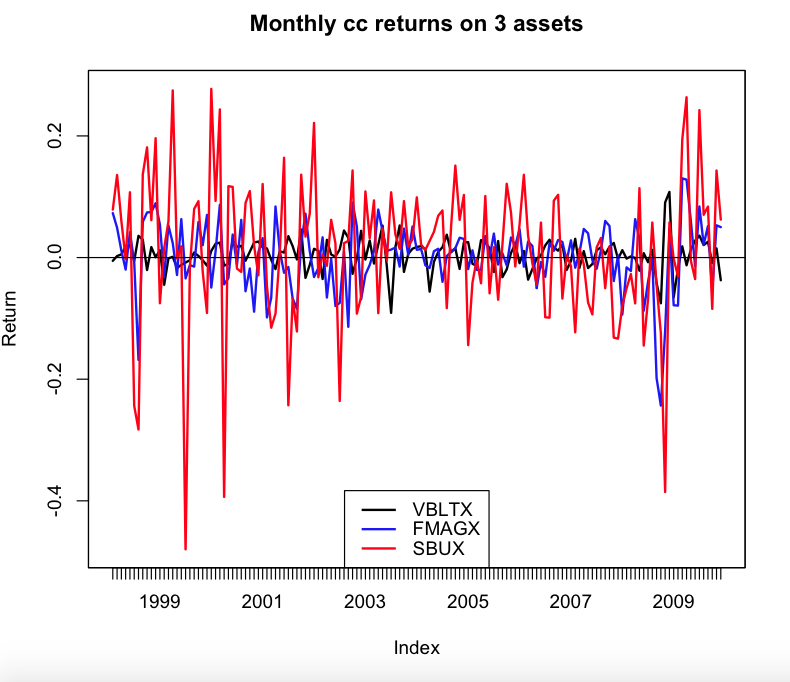
\includegraphics[scale = 0.4]{returns}
The returns appear to look stationary. Returns for the bond fund seem to go up a lot during the crash then fell back down. 
\item 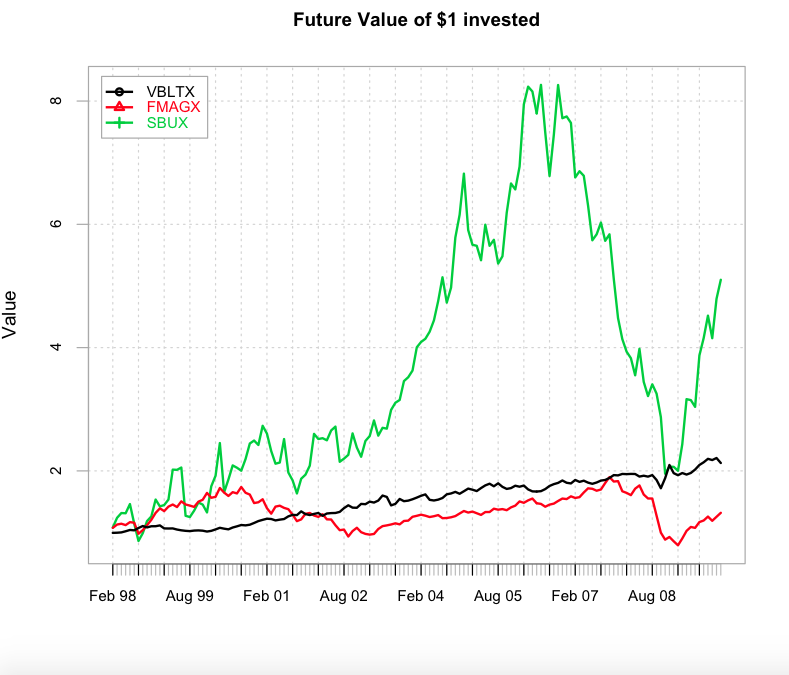
\includegraphics[scale = 0.4]{cumRet}
VBLTX and FMAGX seem to give low returns but with much less volatility. As a result, their returns are lower compared to Starbucks, which has the highest best investment horizon. On the contrary, FMAGX does not look like it has a bright future with the FV crashing and slowly recovering.
\item 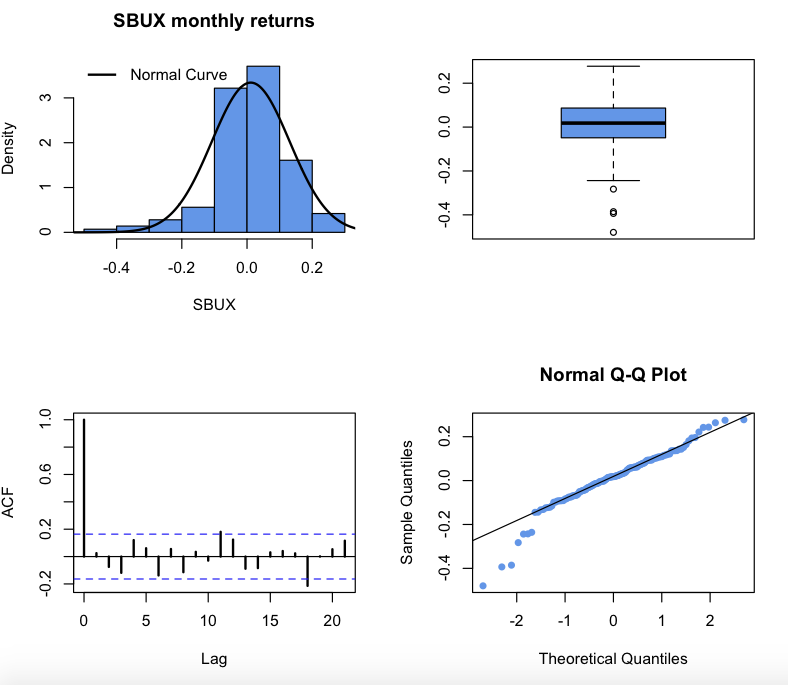
\includegraphics[scale = 0.4]{4}
No the returns do not look normally distributed. The returns look like they are left skewed with heavy tails and extreme outliers.
\item \begin{lstlisting}
                   VBLTX    FMAGX     SBUX
Observations    143.0000 143.0000 143.0000
NAs               0.0000   0.0000   0.0000
Minimum          -0.0909  -0.2434  -0.4797
Quartile 1       -0.0095  -0.0205  -0.0488
Median            0.0086   0.0099   0.0182
Arithmetic Mean   0.0053   0.0019   0.0114
Geometric Mean    0.0049   0.0003   0.0035
Quartile 3        0.0197   0.0396   0.0868
Maximum           0.1079   0.1302   0.2773
SE Mean           0.0022   0.0047   0.0100
LCL Mean (0.95)   0.0010  -0.0074  -0.0083
UCL Mean (0.95)   0.0096   0.0113   0.0311
Variance          0.0007   0.0032   0.0143
Stdev             0.0261   0.0567   0.1194
Skewness         -0.1526  -1.0424  -0.9070
Kurtosis          2.9516   2.6936   2.6917
\end{lstlisting}
It looks like starbucks has the highest median return while VBLTX has the lowest, but it does have the lowest SE mean while SBUX has the highest SE, Varm SD and lowest kurtosis. Therefore, it is most likely the riskiest asset while VBLTX is the least risky asset.
\item \begin{lstlisting}
> 12*apply(ret.mat, 2, mean)
 VBLTX  FMAGX   SBUX 
0.0634 0.0233 0.1367 
> 
> # annualized simple mean
> exp(12*apply(ret.mat, 2, mean)) - 1
 VBLTX  FMAGX   SBUX 
0.0654 0.0236 0.1465 
\end{lstlisting}
There is nothing surprising, the implied simple mean should be greater than the continuously compounded 

\item \begin{lstlisting}
sqrt(12)*apply(ret.mat, 2, sd)
 VBLTX  FMAGX   SBUX 
0.0903 0.1963 0.4137 
\end{lstlisting}
The SD for VBLTX is extremely low while the SD for SBUX is extremely high, likely indicating there are a lot of factors that affect the performance of Starbucks (gas, bean price, economy, etc.)
\end{enumerate}
\vfill \hrule \vspace{2mm} \centerline {\tt \tiny http://computational-finance.uw.edu}
\end{document}